\chapter{Instrumentación electronica y programas de control}
\label{chap:instrumentation}
\textit{En este capítulo se muestra el trabajo realizado para el desarrollo de los programas de control necesarios
para controlar el monocromador HR60 en las mediciones del sistema.}
\vfill
\minitoc
\newpage

\section{Monocromador}
\label{ch2:monochromator}
Las espectroscopias se basan en descomponer la luz que se incide o refleja de un material a estudiar, en un espectro de longitudes de onda para poder facilitar su estudio. Un ejemplo de estas técnicas lo son la \textit{Reflectancia Diferencial Espectroscópica} y la \textit{Espectroscopia Raman}.
 
El monocromador es la parte esencial en los sistemas para medir espectroscopias, ya que su principal función es el controlar o aislar la longitud de onda con la cual se esta censando un espectro de alguna espectroscopia\cite{Murty1974}. Esto se hace por medio de un arreglo de espejos y una \textit{rejilla de difracción}, la cual funge como el elemento dispersor de la luz para obtener el espectro lumínico. Este arreglo es descrito en la Fig. \ref{fig:mono_diagram}.

\begin{figure}[H]
    \centering
    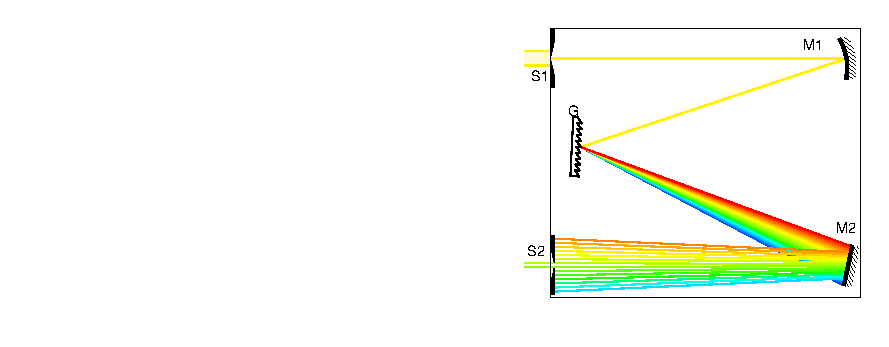
\includegraphics[width=0.6\textwidth]{figures/chap2/mono1.pdf}
        \caption{Diagrama esquemático del monocromador HR60\cite{PdHGaby}, donde \textit{S} son las slits, \textit{M} los espejos fijos y \textit{G} la rejilla de difracción.}
    \label{fig:mono_diagram}
\end{figure}

Cabe destacar, que la Fig. \ref{fig:mono_diagram}, es una representación esquemática del sistema trabajado. $S_{1}$ y $S_{2}$, son las \textit{slits} o aperturas finas controlables, por las cuales regulamos la cantidad de luz en el sistema, para despues incidir en el espejo esférico $M_{1}$, donde es difractada por una \textit{rejilla de difracción}, la cual es móvil en un eje para poder seleccionar la longitud de onda deseada por medio del espejo plano $M_{2}$ y la slit $S_{2}$, la cual proporciona el ancho espectral de nuestro haz de luz.

\section{Electrónica del monocromador HR60}
\label{sec:ch2-electronic}
El uso final del monocromador utilizado será el realizar las espectroscopias de \textit{Reflectancia Diferencial} y \textit{Elipsometria}, por lo que este sistema debe estar automatizado en el movimiento de la \textit{rejilla de difracción} y la apertura de las \textit{slits}, por lo que es crucial que estos sean controlados de forma sencilla y eficaz. Para esto, se utilizan \textit{motores a paso o steppermotor} controlados por una \textit{unidad de control} que usualmente es en base a un microcontrolador, la cual procesa la información proporcionada por un PC para controlar el monocromador. 

La conexión monocromador-PC se hace utilizando la \textit{comunicación serial} utilizando el protocolo \textit{RS232}, la cual se basa en el envio de información \textit{bit por bit} en un cierto periodo de tiempo. Esto parece una desventaja, porque la transmisión de la información es de baja velocidad, pero al utilizar instrucciones cortas y sencillas, podemos establecer una comunicación eficaz entre los sistemas. Una importante característica, es que podemos aprovechar esta propiedad de \textit{bit por bit}, para simplificar la interpretación de las instrucciones.

En las siguientes secciones se mostraran las partes fundamentales del sistema.

\subsection{Unidad de control}
\label{sec:ch2-control-unit}
La unidad de control del monocromador HR60 está compuesta por tres componentes.
\begin{itemize}
    \item \textit{Arduino Uno}. El microcontrolador de elección para interpretar las instrucciones recibidas de la PC de control y enviar notificaciones de estado. Este fue escogido por la facilidad a la hora de implementar el programa de control y la gran cantidad de recursos de \textit{software} y \textit{hardware} que existen para este elemento.
    \item \textit{Driver A4988}. Circuito integrado para el control de motores bipolares en el rango de operación 12-30 V. Este tiene la opcion para realizar fracciones del paso utilizando el concepto de \textit{microstepping}. Usado para el control del motor de la \textit{rejilla de difracción}.
    \item \textit{Adafruit Motor Shield}. Se utilizaron dos de estos kits para el control de los motores de las slits. Estos vienen con la documentación necesaria para su implementación.
\end{itemize}

El \textit{Driver A4988} y \textit{Adafruit Motor Shield}, son utilizados para el control y alimentación de los motores, pero por sí solos no pueden interpretar las instrucciones enviadas por el PC de control, por lo que el encargado de desglosarlas y enviar las notificaciones de estado para indicar si el monocromador está en operación o estático es el \textit{Arduino Uno}.

\subsection{Motores del monocromador HR60}
\label{sec:ch2-motors}

Los motores en el monocromador HR60 son los siguientes:
\begin{itemize}
    \item Motor principal o motor de \textit{rejilla de difracción}. Este es un motor bipolar alimentado por 30 V, el cual hace girar un \textit{tornillo sin fin} donde se encuentra montado la \textit{rejilla de difracción}, obteniendo un espectro de 0-1300 nm, el cual esta limitado por un \textit{limit-switch} al final del sin fin. Este tiene una resolución de paso de 0.1 nm y trabaja en el modo de \textit{half-step}, para mejorar la suavidad en su movimiento.
    \item Slits. El sistema tiene cuatro slits, cada una con un \textit{steppermotor} para el control de la  cantidad de luz en el monocromador, estas tienen un mecanismo de apertura y cierre en un rango de 0-2500 nm. Estas no presentan un sistema para limitar su apertura, por lo que hay que ser cuidadosos al momento de utilizarlas.
\end{itemize}

\section{Diseño del programa de control}
\label{sec:ch2-control}
Para diseñar el programa de control del monocromador con base en Arduino, se tomó el programa de control en el \textit{Laboratorio de Elipsometria Espectroscópica, I.I.C.O., U.A.S.L.P} como apoyo. En este se definen algunas secuencias de control para el movimiento del monocromador, esperando una notificación de estado, además del guardado de la posición final del motor principal del sistema y de cada una de sus slits. Entonces para poder realizar la comunicación PC-Monocromador necesitamos lo siguiente:

\begin{itemize}
    \item La unidad de control debe tener en su código los primeros valores para inicializar el monocromador, como la resolución y el tamaño de paso deseado.
    \item Poder enviar una instrucción a la unidad de control, estas se mantendrán en base a las definidas en el programa de control de la PC hecho en VBasic. En específico, la primera instrucción siempre debe ser el inicializar el monocromador o enviarlo al limite del sin fin, para evitar posibles daños. Esto también nos sirve para probar si existe comunicación serial.
    \item Después de inicializar el monocromador, está a nuestra disposición el movimiento de la rejilla de difracción, el cambio de resolución del monocromador y el control de las slits, este en específico es un ciclo donde se espera una instrucción del PC de forma indefinida.
    \item Al inicio y fin de una operación, la unidad de control siempre debe indicar el estado en el que se encuentra el motor, para evitar saturarlo de instrucciones.
    \item El ciclo mencionado no debe terminar siempre y cuando funcione de forma correcta el sistema, en caso de encontrar un error, terminará el mismo.
\end{itemize}

Para más detalles, el código completo se encuentra en el Apéndice \ref{appendix:arduino} y en la Fig. \ref{fig:mono_flow}, podemos observar el diagrama de flujo del programa de control.
\newpage

\begin{figure}[H]
    \centering
    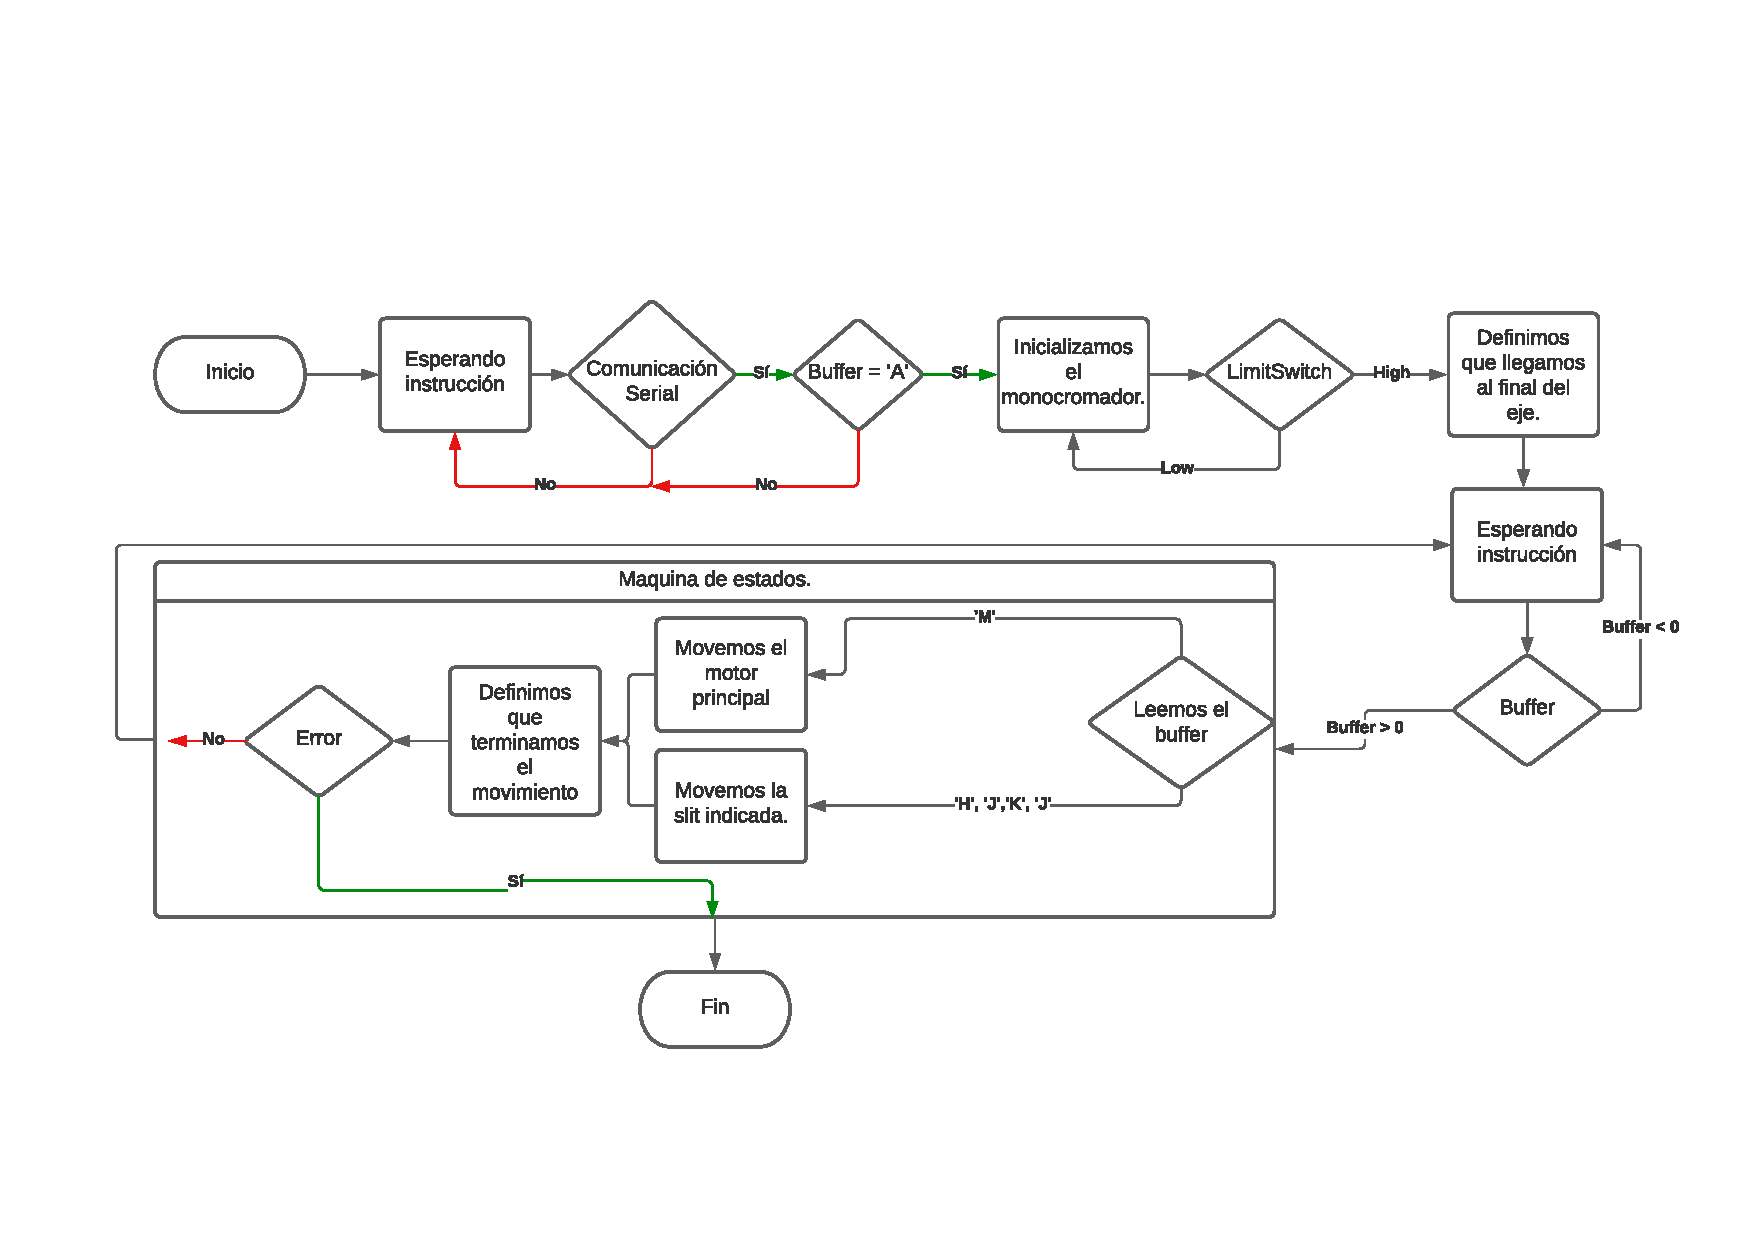
\includegraphics[width=1.5\textwidth, angle=270]{figures/chap2/monocromador.pdf}
        \caption{Diagrama de flujo del programa de control del monocromador}
    \label{fig:mono_flow}
\end{figure}
